\section{Digital ARTVA prototype}
\begin{figure*}
	\centering
	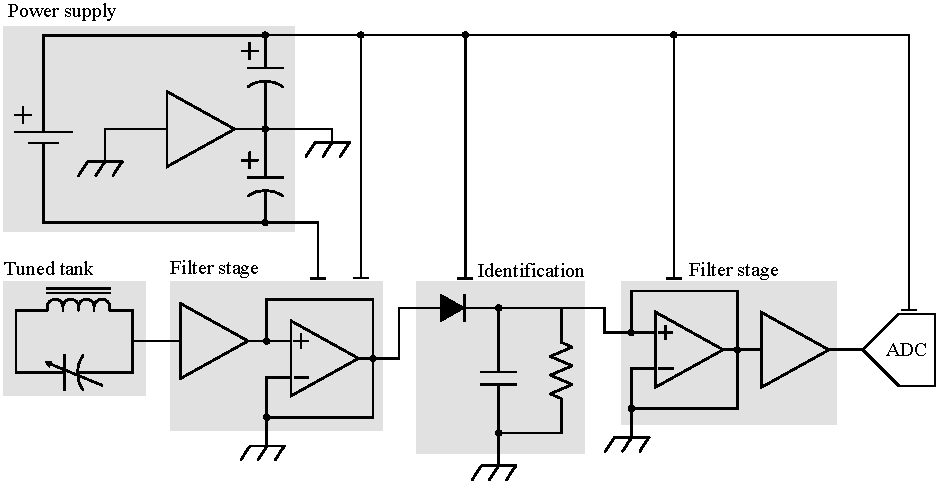
\includegraphics[scale=0.7]{ch2/img/block_circuit.pdf}
	\caption{Block diagram for the circuit}
	\label{fig:block_circuit}	
\end{figure*}
In the last section of this chapter, we use the knowledge collected to develop a prototype of an ARTVA receiver, in which there is not a transmission part. The receiver is the only fundamental module that we need for our drone, a transmitter will only be useless weight. 

In figure \ref{fig:block_circuit} there is the block outline of the device:
\begin{itemize}
\item the first block is the tuned tank, or tuned amplifier
\item the second block is the buffer and pre--amplifier
\item the third block is the identification part
\item an amplification and a second buffer
\item digital component
\item dual supply stage
\end{itemize}
Through this section, each block will be discussed and explained. The design process has taken into account the tolerances for passive components\sidenote{Resistors: 5\%\newline Capacitors: 20\%}, but nothing can be done for thermal derive, that increases tolerance ranges to almost unpredictable values.

\subsection{Tuned tank}
% \begin{figure}[b]
% 	\includegraphics[viewport=x y x y]{ch2/img/receiver3.pdf}
% 	\caption{}
% 	\label{fig:circuit}
% 	%\forceversofloat
% \end{figure}
\begin{figure}[h]
	\centering
	\includegraphics*[viewport=3 3 240 457,scale=0.4]{ch2/img/receiver3.pdf}
	\caption{Tuned tank portion of circuit}
	\label{fig:tunedtank}
	%\forceversofloat
\end{figure}

The tuned tank is composed by a ferrite antenna, with a rod of \num{10}\si{\centi\meter} per \diameter \num{1}\si{\centi\meter}. The wire of the coil is a \num{30} AWG enameled copper wire, with a final parasite resistance of \num{22}\si{\ohm}. The coil has \num{70} windings. For more informations about this tuned circuit, check previous section.

\subsection{Buffer and pre--amplification}
\begin{figure*}[h]
	\centering
	\includegraphics*[viewport=170 3 1250 380,scale=0.4]{ch2/img/receiver3.pdf}
	\caption{Pre--amplifier stage}
	\label{fig:filter1}
	%\forceversofloat
\end{figure*}

This block is composed by a first stage that acts as a separation between the tuned tank and the filter, also called voltage follower. To limit the number of components on the board this stage is obtained with an operational amplifier. To grant a longer receiving range, an high--gain selective active filter is in cascade to the buffer before the identification and acts as a pre--amplifier. It is important to select an operational amplifier with an high bandwidth--gain--product to grant the gain at \num{457}\si{\kilo\hertz}, at which the filter is centered. Also, this stage depends to the dual \num{\pm 5}\si{\volt} supply stage. 
\begin{marginfigure}
	\centering
	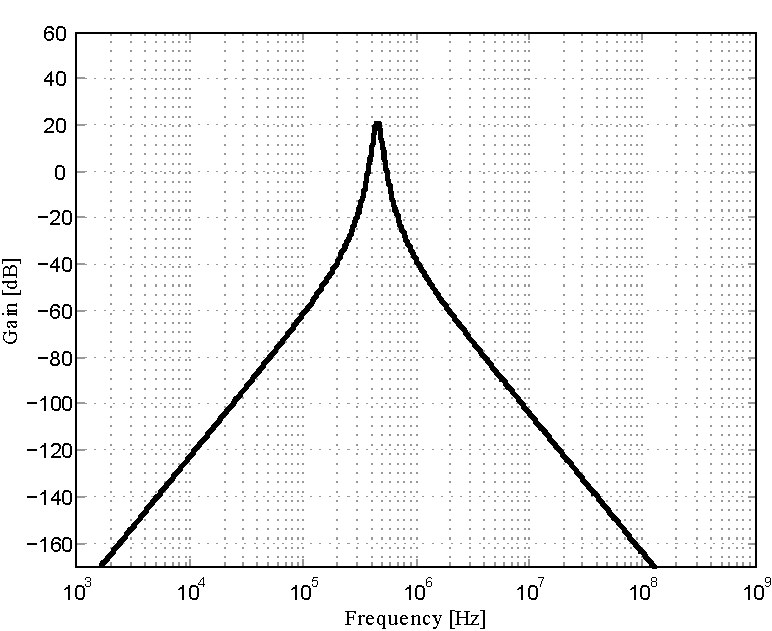
\includegraphics[width=5cm]{ch2/img/filter1.pdf}
	\caption{Filter magnitude characteristic}
\end{marginfigure}

The op--amp chosen is \texttt{LF347N}, even if a faster amplifier may be selected, it is advised to stay below the \num{60}\si{\mega\hertz} BW, to avoid auto--resonance effects.

\subsection{Identification}
\begin{figure}[h]
	\centering
	\includegraphics*[viewport=1251 3 1580 595,scale=0.4]{ch2/img/receiver3.pdf}
	\caption{Identification stage}
	\label{fig:identifier}
	%\forceversofloat
\end{figure}
\begin{marginfigure}
	\centering
	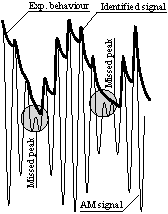
\includegraphics[width=4.5cm]{ch2/img/identificatore.pdf}
	\caption{Logical function of an identifier}
	\label{fig:identifier_log}
\end{marginfigure}
The central block is an identification circuit, obtained with the monolithic classical IC \texttt{TA7641}\sidenote{A.k.a.: \texttt{MK484} evolution of \texttt{ZN414}},  that acts as a one chip radio solution in AM. All receiver is derived from the modification of the basic circuit provided in schematics of this IC, extended with filtering and buffers, and the removal of the auto gain control resistance in the output feedback. Also, transistor amplification stage is removed. The output of this circuitry is in \numrange{40}{60}\si{\milli\volt}, with a very low current required. The input pin has a good impedance 

To better understand the use of this stage, look at figure \ref{fig:identifier_log}, in which an extremely simplified version of the IC behavior is represented with common components that are drawn in figure \ref{fig:block_circuit}. The IC straightens the received signal and identifies the envelope of the modulated intelligence with a low pass filter that has a dynamic not too slow, to not loose some of the higher frequencies information modulated (also called missed peak). IC implements this function with an high quality envelope detector.
\begin{figure*}[h]
	\centering
	\includegraphics*[viewport=1443 3 2320 350,scale=0.4]{ch2/img/receiver3.pdf}
	\caption{Low pass filter and amplification stage}
	\label{fig:filter2}
	\forcerectofloat
\end{figure*}

\subsection{Amplifier}

The identified signal is, again, amplified and filtered, to a lower frequency, to grant the isolation of the square wave, with respect to the residual carrier and other source of interference. A \num{10}\si{\decibel} gain filter, with 2 stages was implemented. After the filter, another buffer connects analog circuitry with digital micro--controller.
\begin{marginfigure}
	\centering
	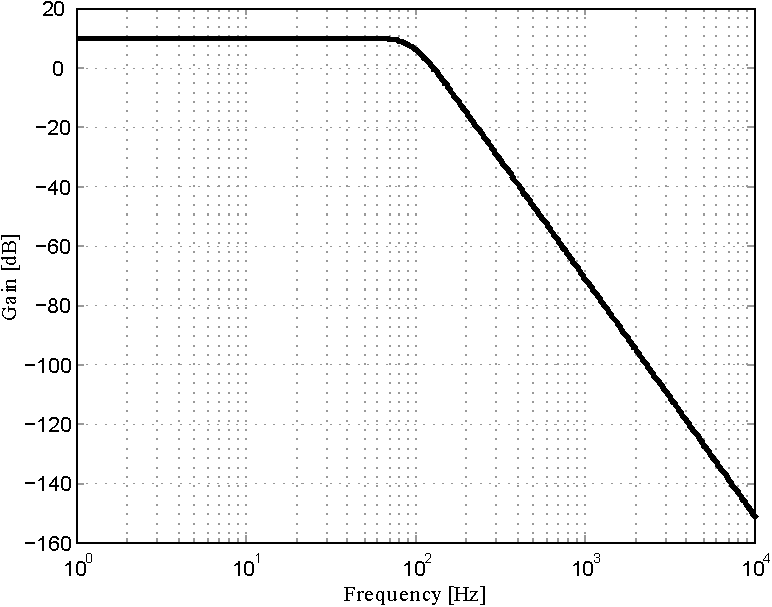
\includegraphics[width=5cm]{ch2/img/filter2.pdf}
	\caption{Filter magnitude characteristic}
\end{marginfigure}

\subsection{Digital stage}
\begin{figure}[h]
	\centering
	\includegraphics*[viewport=2320 3 2650 350,scale=0.4]{ch2/img/receiver3.pdf}
	\caption{Digital stage}
	\label{fig:adc}
	%\forceversofloat
\end{figure}
One last stage is the ADC and the UART interface on the micro--controller. Using an \texttt{MSP430} it is easy to develop in \texttt{C} the routines necessary to perform the task. To reduce the power consumption, ADC sampling is performed with ALU in power saving mode. Once the sampling task is completed, an interrupt brings up the ALU that set up the variables too be sent over serial interface UART (or SPI or I2C).

\subsection{Dual supply}
The supply is obtained through the use of a virtual ground and a symmetrical classical regulation circuit. This scheme is sometimes called rail splitter, and it is necessary for the first regulation stage, to avoid op--amps saturation.
\begin{figure}[h]
	\centering
	\includegraphics*[viewport=3 450 580 750,scale=0.4]{ch2/img/receiver3.pdf}
	\caption{Example of a sampling result}
	\label{fig:sampling_res}
	\forceversofloat
\end{figure}

\subsection{Tri--axes ARTVA}
In figure \ref{fig:sampling_res} there is an example of sampling from the real prototype, using MATLAB serial reading capabilities. A complete prototype uses three equal antenna--filter--identification--amplifier stage, with orthogonal antennas, and one single ADC micro--controller and power supply unit.
\begin{figure}[h]
	\centering
	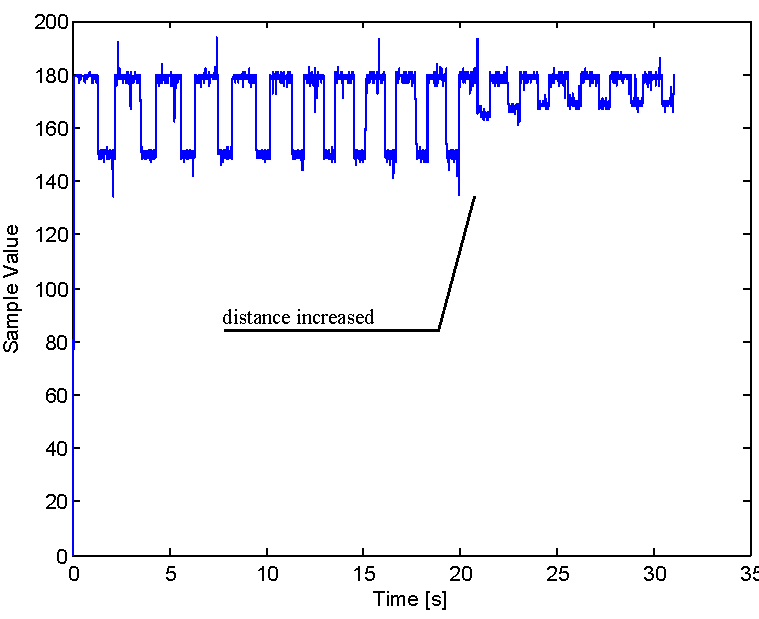
\includegraphics[scale=0.6]{ch2/img/sampling_result.pdf}
	\caption{Complete circuit}
	\label{fig:samplig_res}
	%\forceversofloat
\end{figure}
\begin{figure}[h]
	\centering
	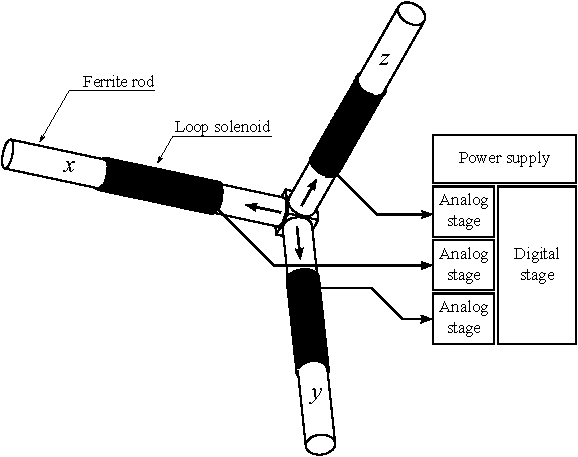
\includegraphics[scale=0.8]{ch2/img/triplantenna.pdf}
	\caption{Triple antenna}
	\label{fig:trantenna}
	%\forceversofloat
\end{figure}
\begin{figure}[p]
	\centering
	\includegraphics[scale=0.25,angle=90]{ch2/img/receiver3.pdf}
	\caption{Complete circuit}
	\label{fig:completecirc}
	\forceversofloat
\end{figure}